
\section{Simulation flow follow-up \ddcnew}
\label{chap5_newFlow}
Due to the shortcomings of the simulation flow presented in chapter \ref{chap:3icModeling}, which mainly lie in the fact that a hundred of transistors is approximated with two resistors and four capacitors, the simulation flow follow-up aims at considering the logical function of some of these transistors.
To that end, one has to first choose a target \scs where they want to conduct the further analysis.
Then, the \scs internal signals are extracted from the \scs simulation, and then they can be injected into simulated logic gates.
The main signals of use are the following:
\begin{itemize}
    \setlength\itemsep{-0.1em}
    \item VDD: the positive power supply net;
    \item VSS: the negative power supply net;
    \item VEPI: the voltage at the epitaxy level, also known as the junction between the substrate and the top of the \scs;
    \item VNW (VGP): the N-well voltage, required in both \dwF and \twF substrates;
    \item VPW: the P-well voltage, only required in a \twF substrate.
\end{itemize}
The signals VEPI, VGP, VPW and VNW, depending on the substrate type, act as the bulk voltage of the simulated transistors.
In line with VDD and VSS, the shape of these signals dynamically change the bias of the transistors, and therefore their temporal behavior.
To have a comprehensive understanding of the various possible scenarios, in addition to keeping clarity, I present the results for logic inverters, composed of two transistors in the technology of my thesis target microcontroller: 90 nm bulk.
\twF and \dwF substrates are presented in this order, and for each substrate type, two inverters are simulated: a normally low and a normally high.
The simulated schematic and their significant signals are shown in Fig. \ref{fig_ivxSim}.

%\begin{figure}[ht]
%    \centering
%    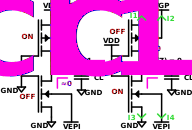
\includegraphics[width=0.5\textwidth]{5_faultModel/figures/ivx3NewNoSignals.pdf}
%    \caption{PLACEHOLDER.}
%    \label{fig_ivxNoSig}
%\end{figure}

\begin{figure}[ht]
    \centering
    \begin{subfigure}{0.47\textwidth}
        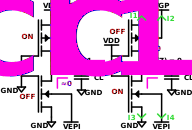
\includegraphics[width=1.0\textwidth, center]{5_faultModel/figures/ivx3NewNoSignals.pdf}
        \caption{PLACEHOLDER.}
        \label{fig_ivxNoSig}
    \end{subfigure}
    \hfill
    \begin{subfigure}{0.47\textwidth}
        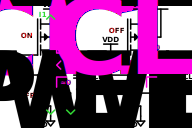
\includegraphics[width=1.0\textwidth, center]{5_faultModel/figures/ivx3New.pdf}
        \caption{PLACEHOLDER.}
        \label{fig_ivxSig}
    \end{subfigure}
    \caption{PLACEHOLDER.}
    \label{fig_ivxSim}
\end{figure}

For each scenario, I present five signals of interest:
\begin{itemize}
    \setlength\itemsep{-0.1em}
    \item The voltage pulse at the IC backside, for reference purposes (in orange);
    \item The local power supply voltage seen by the transistors (in black);
    \item The current sum of the inverter of interest (in medium green);
    \item The load current of the inverter of interest (in magenta);
    \item The output of the normally high inverter (in light cyan);
    \item The output of the normally low inverter (in dark blue);
    \item The P-well (otherwise epitaxy) voltage (in dark cyan);
    \item The N-well (otherwise VGP) voltage (in dark yellow).
\end{itemize}
Concerning the \twF substrate, the inverter of interest is the normally high one, while for the \dwF substrate, it is the normally low one.

%The main shortcoming of the simulation flow presented in chapter \ref{chap:3icModeling} lies in the fact that the models do not consider the logic functions of the considered ICs.
%To that end, I introduce in this section a way to circumvent this limitation.
%As the \scs models are made for a specific technology, in that case for a 90 nm bulk silicon manufacturing process, the models parameters are calculated according to this technology node.
%In addition to this, a single \scs model represents a hundred of logic gates.
%Therefore, the disturbances observed in a \scs elementary block are the ones these logic gates would be subject to during \bbi.
%With this in mind, I chose a very simple method of using the data from \scs simulations.
%
%It consists in modeling actual transistors and logic gates with the considered technology and simulating them using the extracted disturbances from the \scs simulation results.
%For the purpose of this work, I chose to simulate inverters in two specific scenarios:
%\begin{itemize}
%    \setlength\itemsep{-0.1em}
%    \item A normally low inverter, fed with a logical high signal at its input;
%    \item A normally high inverter, fed with a logical low signal at its input.
%\end{itemize}
%
%
\begin{figure}[ht]
    \centering
    \begin{subfigure}{0.48\textwidth}
        \includegraphics[width=1.0\textwidth, center]{5_faultModel/figures/logic_gates_solo_M0_DW.pdf}
        \caption{PLACEHOLDER.}
        \label{fig_ivxDual}
    \end{subfigure}
    \hfill
    \begin{subfigure}{0.48\textwidth}
        \includegraphics[width=1.0\textwidth, center]{5_faultModel/figures/logic_gates_solo_M0_TW.pdf}
        \caption{PLACEHOLDER.}
        \label{fig_ivxTriple}
    \end{subfigure}
    \caption{PLACEHOLDER.}
    \label{fig_ivxSimRes}
\end{figure}
